\documentclass{hw}

\title{CS 5220 -- Project 3: Shortest Paths}
\author{Group 10: Ze Jin (zj58), Ben Shulman (bgs53), Michael Whittaker (mjw297)}
\date{\today}
\rhead{Group 10}

\usepackage{caption}
\usepackage{fancyvrb}
\usepackage{subcaption}

\newcommand{\secref}[1]{Section~\ref{sec:#1}}
\newcommand{\icc}{\texttt{icc}}

\newcommand{\rs}{\textsc{rs}}
\newcommand{\rsomp}{\textsc{rs-omp}}
\newcommand{\rsmpi}{\textsc{rs-mpi}}
\newcommand{\rshybrid}{\textsc{rs-hybrid}}

\newcommand{\block}{\textsc{block}}
\newcommand{\blockomp}{\textsc{block-omp}}
\newcommand{\blockmpi}{\textsc{block-mpi}}
\newcommand{\blockhybrid}{\textsc{block-hybrid}}

\newcommand{\fw}{\textsc{fw}}
\newcommand{\fwomp}{\textsc{fw-omp}}
\newcommand{\fwmpi}{\textsc{fw-mpi}}
\newcommand{\fwhybrid}{\textsc{fw-hybrid}}

\begin{document}
\maketitle

\section{Introduction}\label{sec:intro}

In this project, we analyze the OpenMP version of Floyd-Warshall algorithm by profiling the code using Vtune to identify bottlenecks. The Vtune profiling result is shown in section \secref{profiling}. To tune the code, we explore different compiler flags (section \secref{compilerflags}) and slightly vectorized the code (section \secref{vectorization}). Finally we perform strong and weak scaling in section \secref{evaluation}. 
\section{Profiling}\label{sec:profiling}
\subsection{Identify bottlenecks}
To define the bottlenecks of \ttt{path.C}, we profiled our code
using Intel's VTune Amplifier to understand which part of the code takes the most time to run. VTune Amplifier commands is shown in \figref{amplxe-command}.

\begin{figure}[h]
	\footnotesize
	\begin{verbatim}
	amplxe-cl -collect advanced-hotspots ./path
    amplxe-cl -R hotspots -report-output vtune-report.csv -format csv -csv-delimiter comma
	\end{verbatim}
	\caption{VTune Amplifier Command}
	\label{fig:amplxe-command}
\end{figure}

\subsection{Initial Timing Result}
As shown in \figref{initial-profile-result}, the majority of time is spent inside the \ttt{sqaure} function. We will take about how we optimize the performance of the \ttt{square} function in \secref{vectorization}.  

\begin{figure}[h]
	\footnotesize
	\begin{verbatim}
	Function                     Module        CPU Time		CPU Time:Ideal
	-----------------------------------------  --------     --------------
	square			           	 path.x         45.14s			39.03s
	_kmpbarrier                  libiomp5.so    6.485s			 0.16s
	_kmpc_reduce_nowait          libiomp5.so    2.979s			 	0s
	_kmp_fork_barrier            libiomp5.so    2.553s			 0.03s
	gen_graph             		 path.x         0.030s				0s
	_intel_ssse3_memcpy          path.x         0.030s				0s
	fletcher16                   path.x         0.030s				0s
	\end{verbatim}
	\caption{Initial Profile Result}
	\label{fig:initial-profile-result}
\end{figure}

\section{Algorithms}\label{sec:algo}
In this section, we describe the three algorithms we implemented to compute
all-pairs shortest paths.

\subsection{Repeated Squares}
The release implementation uses a simple repeated squares (\rs) dynamic
programming algorithm. Let $l_{ij}^s$ represent the length of the shortest path
from vertex $i$ to vertex $j$ of at most length $2^s$. \rs{} relies on the
following recurrence:
\[
  l_{ij}^{s+1} = \min_k \group{l_{ik}^s + l_{kj}^s}
\]
The base case $l_{ij}^0$ is the weight of the edge from vertex $i$ to vertex
$j$ or $\infty$ if no such edge exists. This recurrence is nearly identical to
the formula used to compute the square of a matrix $A$:
\[
  a_{ij}^2 = \sum_k a_{ik} a_{kj}
\]

The algorithm initializes the distance matrix $L^s$ for $s=0$ and iteratively
computes $L^{s+1}$ by squaring $L^s$. The algorithm terminates once squaring
$L$ reaches a fixpoint; that is, once $L^2 = L$. Each squaring requires
$O(N^3)$ operations where $N$ is the number of vertices in the graph and the
side-length of $L$. A shortest path can be of at most length $N$, so the
algorithm terminates after at most $\log N$ iterations. Thus, the running time
of \rs{} has a worst-case running time of $O(N^3 \log N)$.

\subsection{Blocked Repeated Squares}
The release implementation of \rs{} uses a naive matrix multiplication kernel
to square $L$. We developed an optimized matrix multiplication kernel that
implements a variety of optimizations. We use this kernel in an optimized
repeated squares implementation that we call \block{}. In this subsection, we
describe the optimizations implemented by \block{}.

\paragraph{Blocking}
A naive matrix multiplication kernel has very poor cache locality. \block{}
implements a blocked matrix multiplication to greatly improve cache locality.
An optimal block size of 128 was found empirically.

\paragraph{Copy Optimization}
When \block{} multiplies two sub-blocks, it first copies them into a smaller,
aligned buffer. This copy optimization allows the compiler to more aggressively
vectorize loops over the sub-blocks and it makes memory accesses to the
sub-blocks much more regular.

\paragraph{Compile-Time Loop Bounds}
If the size of a matrix is not divisible by the size of a block, then not all
sub-blocks will have the same size, and the size of a sub-blocks is only known
at runtime. When \block{} multiplies two sub-blocks, it first checks to see if
they are full-sized blocks, and if they are, it multiplies them using a kernel
whose loop bounds are known at compile-time. By knowing loop-bounds at compile
time, the compiler more aggressively optimizes this code path.  If the
sub-blocks are not full-sized blocks, then it multiplies them using loops with
bounds known at runtime. Since most blocks are full-sized blocks, \block{}
often performs block multiplication with the fully optimized kernel.

\paragraph{Vectorization}
\block{} organizes all loops and array accesses to be fully vectorized.

\subsection{Floyd-Warshall}
The Floyd-Warshall algorithm (\fw{}) is a dynamic programming algorithm
developed by Robert Floyd and Stephen Warshall in the 1960's. Consider a
directed graph  with $N$ nodes ordered $1, \ldots, N$. Let $l_{i,j}^k$ be the
length of the shortest path from vertex $i$ to vertex $j$ using only
intermediate nodes from $\set{1, \ldots, k}$ or $\infty$ if no such path
exists. \fw{} relies on the following recurrence:
\[
  l_{i,j}^{k+1} = \min \group{l_{i,j}^k, l_{i,k+1}^k + l_{k+1,j}^k}
\]
The base case $l_{i,j}^0$ is the weight of the edge from vertex $i$ to vertex
$j$ or $\infty$ if no such edge exists. \fw{} initializes $L^k$ for $k=0$ and
iteratively computes $L^{k+1}$ from $L^{k}$ using the above recurrence.
$L^{k+1}$ can be computed in $O(N^2)$ time and the algorithm terminates when it
computes $L^N$. Thus, the algorithm runs in $O(N^3)$ time.

\section{Parallelization}\label{sec:parallelization}
We parallelized the \rs{}, \block{}, and \fw{} algorithm using three
parallelization mechanisms: OpenMP, MPI, and a hybrid of the two. In this
section, we describe in detail how each mechanisms was used for parallelization.

\subsection{OpenMP}
Parallelizing each algorithm is simply a matter of using \texttt{\#pragma omp
parallel for} before each outer loop of each algorithm's respective square
functions. The implementations of this algorithm are in \texttt{rs-omp.c},
\texttt{block-omp.c}, and \texttt{fw-omp.c}.

\subsection{MPI}
Implementing the algorithms in MPI requires decomposing the problem into sub
parts, similar to the idea of domain decomposition from the last project. We
drew inspiration from previous work with distance-vector routing using
Bellman$-$Ford in determining shortest distances between routers. In that
algorithm, each router sends its distances to all other routers (each time
there is a change) to its neighbors which then use that information to update
their own distances. This continues until no routers have changed distances.

In our case we do not necessarily have a single thread per node, as there maybe
not be enough available hardware threads. Instead each ``router'' is an MPI
rank and is responsible for a set of nodes rather than a single node. Each MPI
rank calculates the minimum distance to each of its nodes from all other nodes
going through each node between 1 and $N$.

For \rs{} and \block{} each rank also determines if any distances have changed.
All MPI ranks then synchronize, to gather distances from one another and
determine if any distances have changed (if none stop then we are done and the
``master'' rank (rank 0) outputs checksum and timing information). To determine
if any distances have changed we use \texttt{mpi\_allreduce} on each rank's done
variable. To synchronize distances across all ranks we use
\texttt{mpi\_allgather} which sends each rank's distances to all other ranks and
collects them from every rank, including itself, into a single buffer. In the
case of \fw{} must synchronize for every iteration of $k$, and does not need to
check if its finished as the algorithm will always finish in the same number of
loops (N). Our implementations are in \texttt{rs-mpi.c}, \texttt{block-mpi.c},
and \texttt{fw-mpi.c}.

\subsection{Hybrid} MPI and OMP interact seamlessly when put together, making it
easy to combine our MPI implementation and the origin OMP implementation. Given
a fixed number of MPI ranks, $r$, and $p$ available threads then each MPI rank
will have access to $p/r$ threads which can be used in OMP parallel sections of
code. This can mean we do not take full advantage of all threads available to us
if $p$ is not divisible by $r$. We implemented a hybrid version of each
algorithm (by combining our MPI implementation and the OMP parts of the original
implementation) in \texttt{rs-hybrid.c}, \texttt{block-hybrid.c}, and \texttt
{fw-hybrid.c}.

\section{Evaluation}\label{sec:eval}

We evaluated our mpi, hybrid implementations of each algorithm (rs, block, fw) by doing strong scaling studies across a range of problem sizes. For rs and block we used a baseline of \rs{omp} and for fw we used a baseline of \fw{omp}. For rs and block we also did weak scaling studies for with a constant work of problem size $n=500$.

\subsection{RS}

\subsubsection{MPI}

\begin{figure}[ht]
\centering
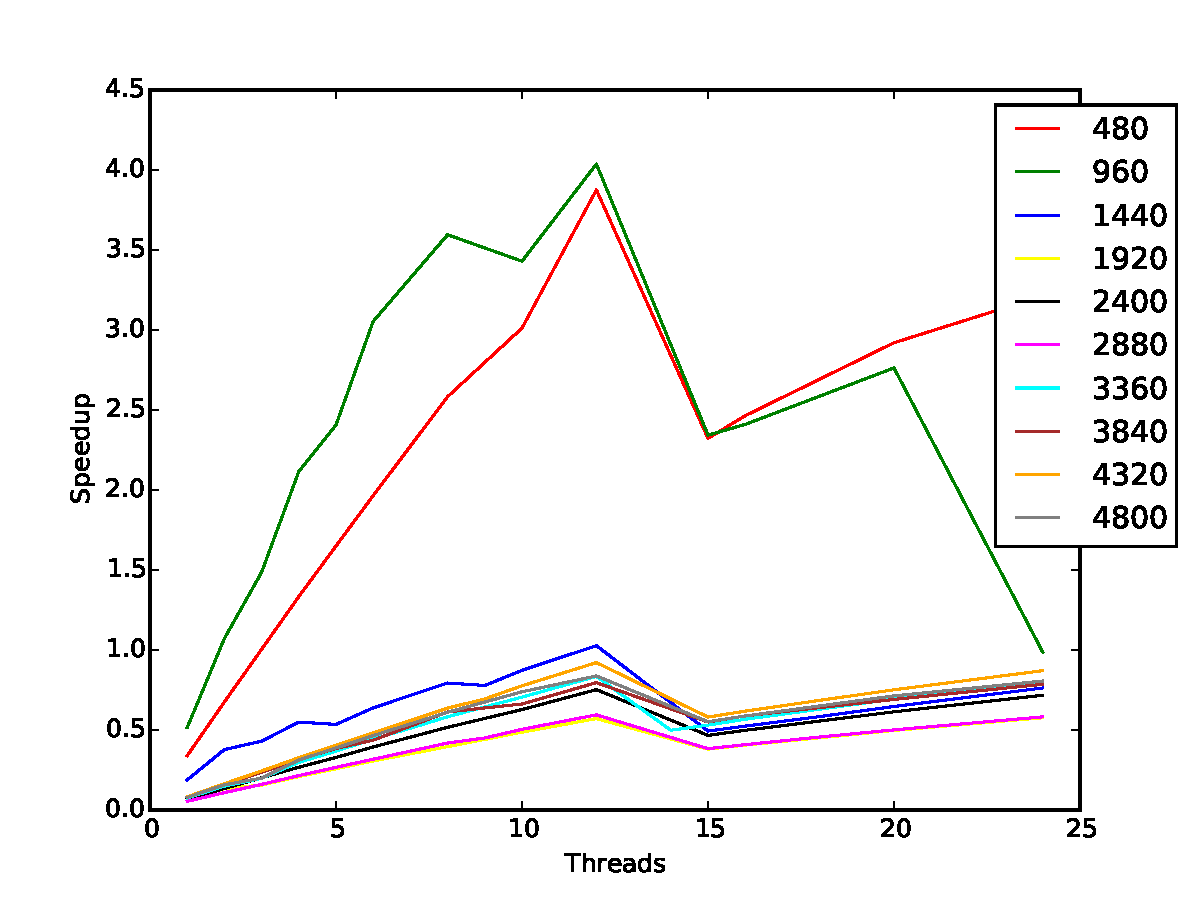
\includegraphics[width=0.5\textwidth]{plots/strong_rs-mpi_baseline-rs-omp--1.pdf}
\caption{Strong scaling for rs-mpi with a baseline of rs-omp}
\label{strong-rs-mpi}
\end{figure}

\begin{figure}[ht]
\centering
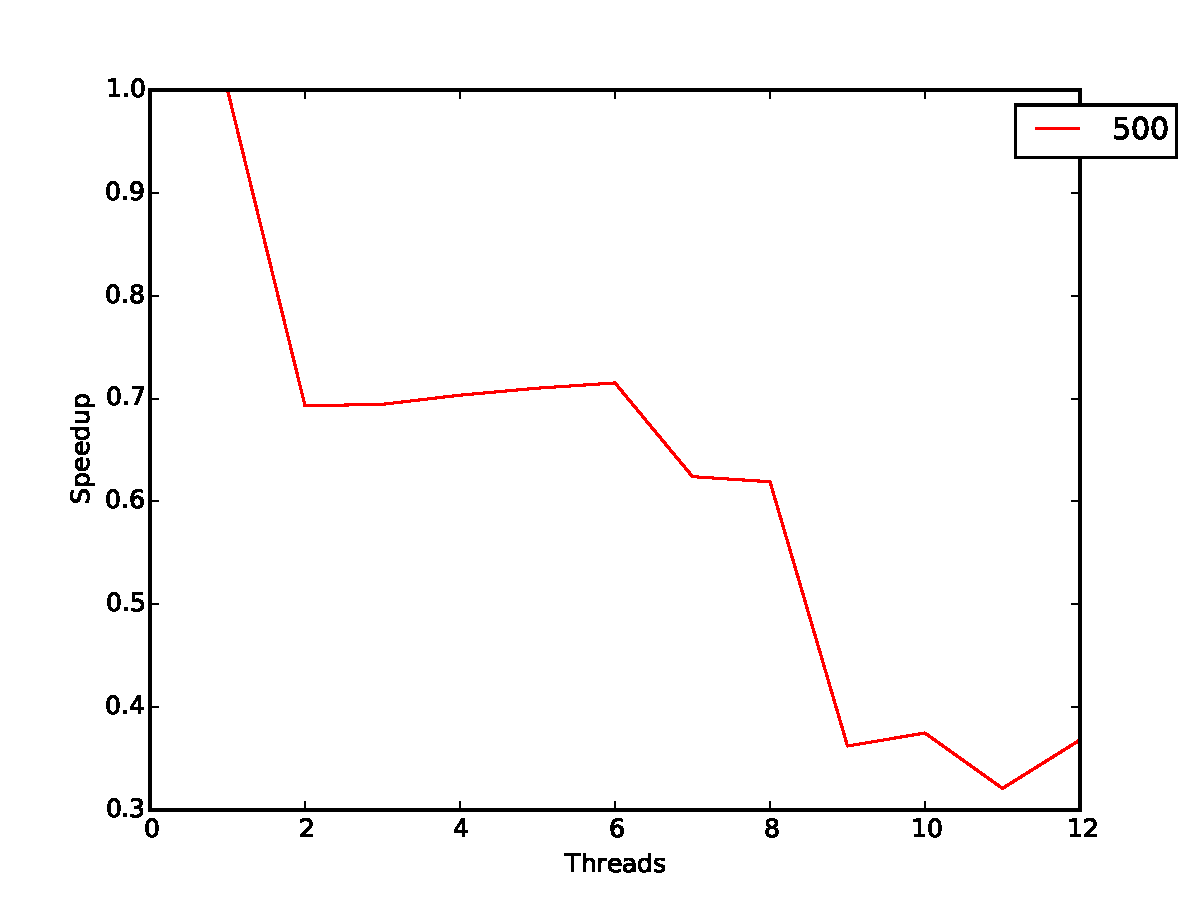
\includegraphics[width=0.5\textwidth]{plots/weak_rs-mpi.pdf}
\caption{Weak scaling for rs-mpi (baseline of itself).}
\label{weak-rs-mpi}
\end{figure}

\subsubsection{Hybrid}

\begin{figure}[ht]
\centering
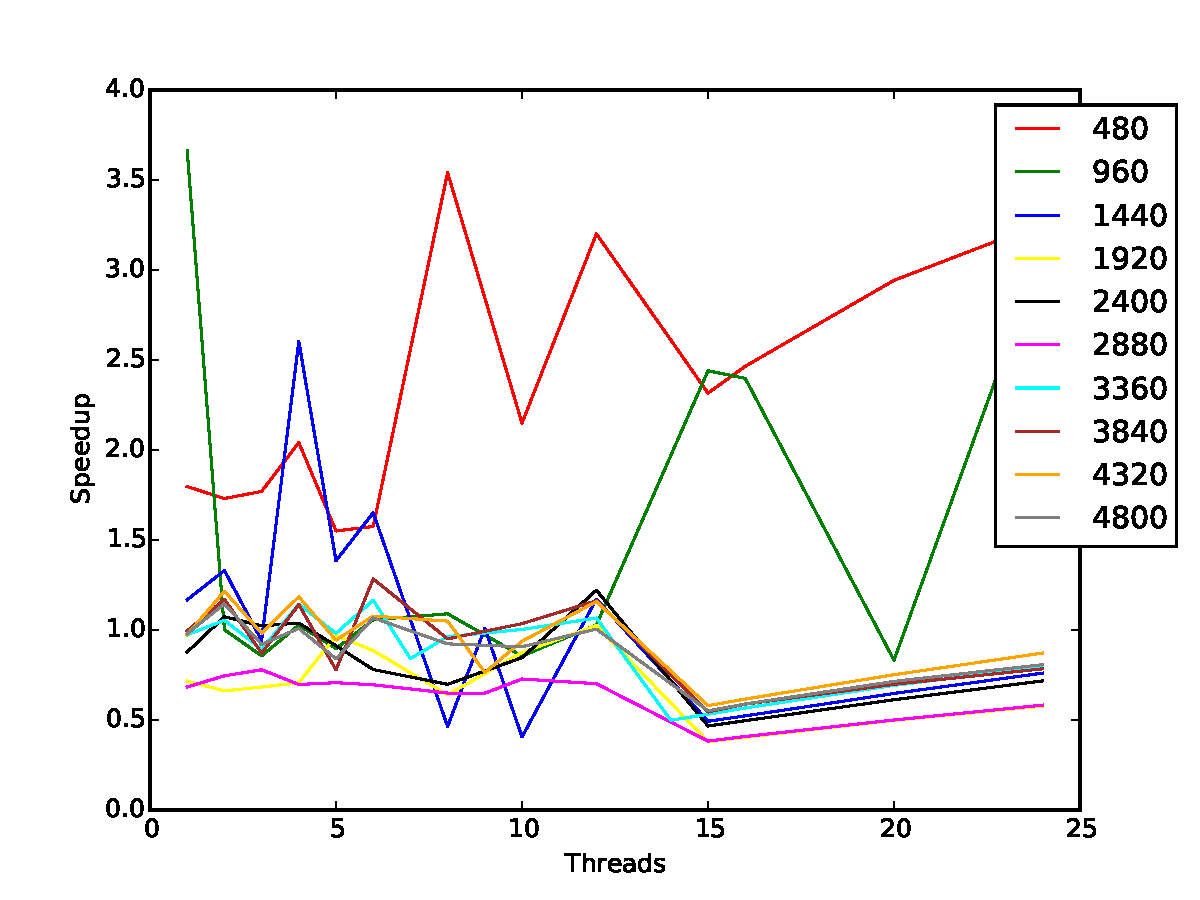
\includegraphics[width=0.5\textwidth]{plots/strong_rs-hybrid_baseline-rs-omp--1.pdf}
\caption{Strong scaling for rs-hybrid with a baseline of rs-omp}
\label{strong-rs-hybrid}
\end{figure}

\begin{figure}[ht]
\centering
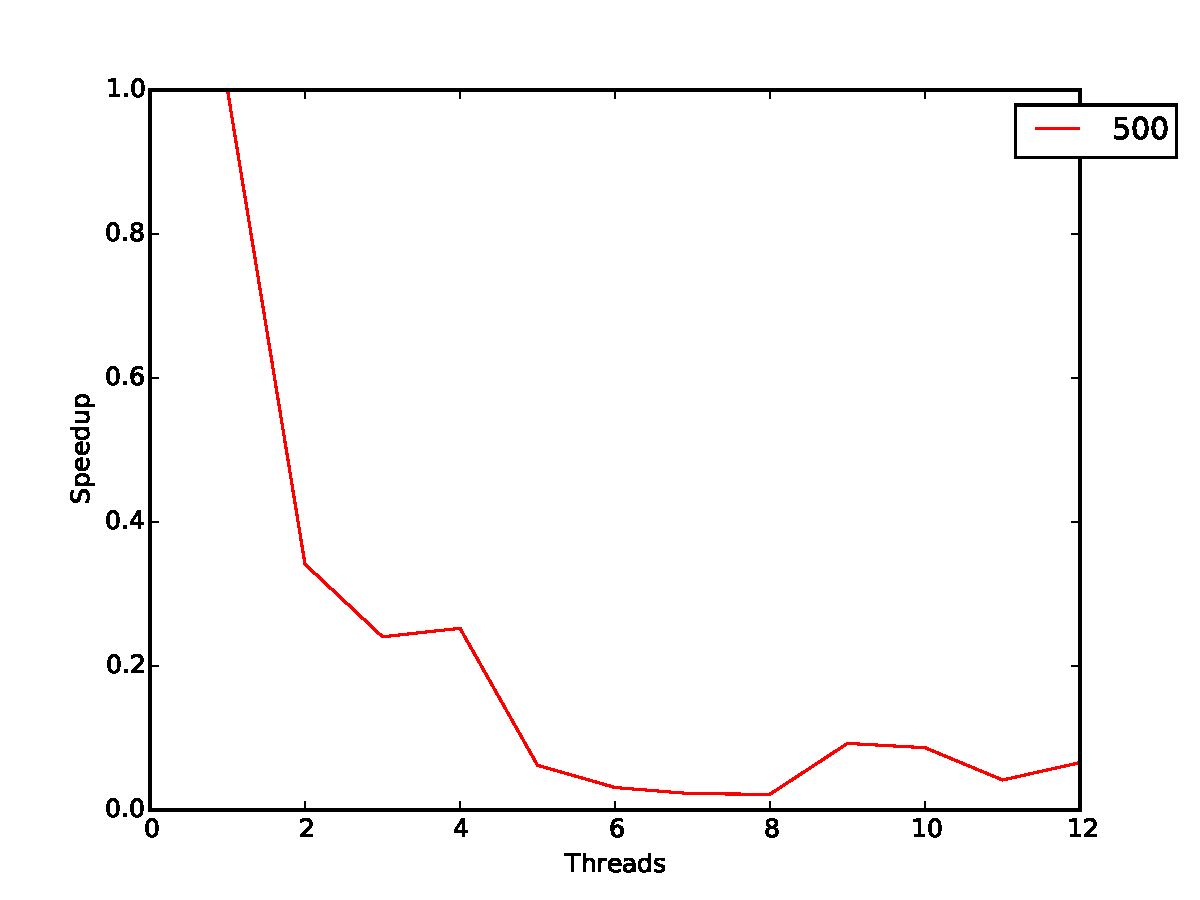
\includegraphics[width=0.5\textwidth]{plots/weak_rs-hybrid.pdf}
\caption{Weak scaling for rs-hybrid (baseline of itself).}
\label{weak-rs-hybrid}
\end{figure}


\subsection{Block}

\subsubsection{MPI}

\begin{figure}[ht]
\centering
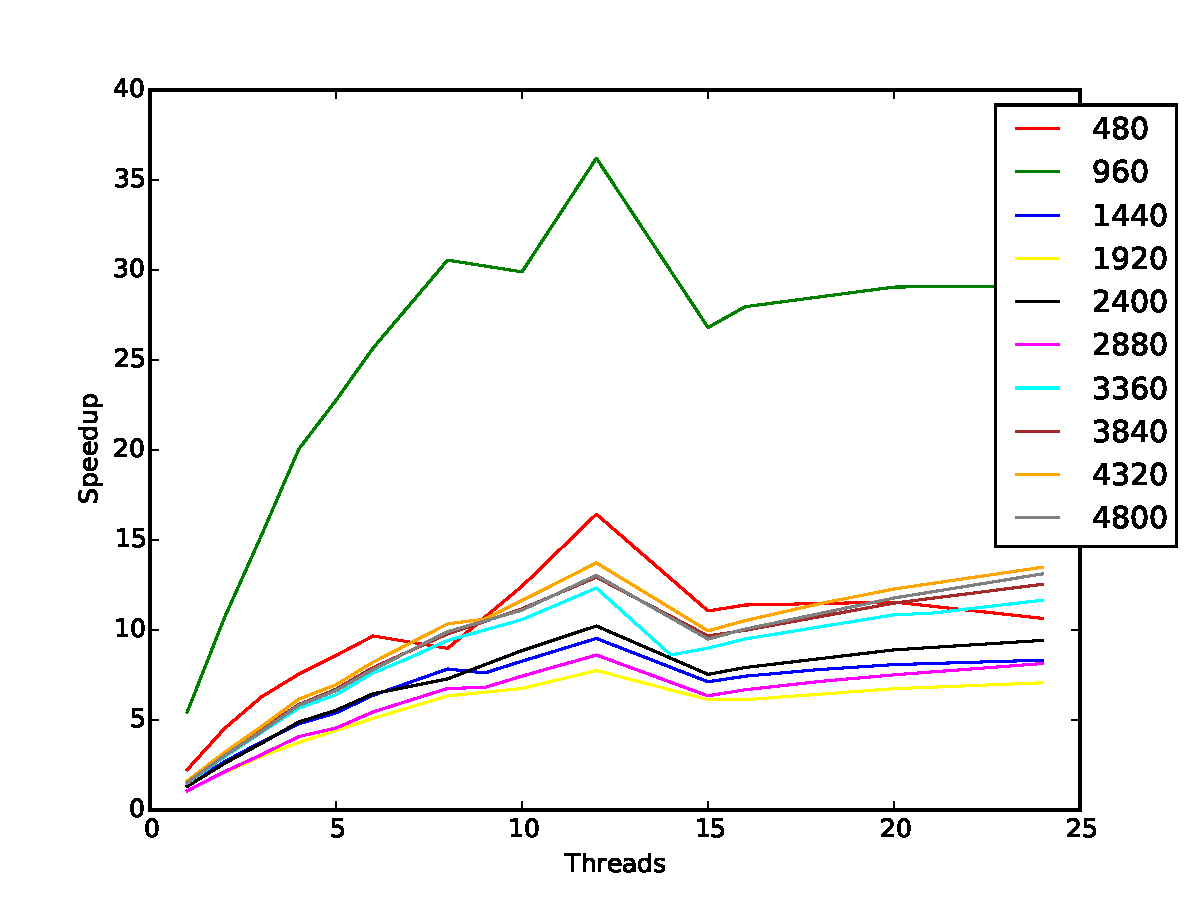
\includegraphics[width=0.5\textwidth]{plots/strong_block-mpi_baseline-rs-omp--1.pdf}
\caption{Strong scaling for block-mpi with a baseline of rs-omp}
\label{strong-block-mpi}
\end{figure}

\begin{figure}[ht]
\centering
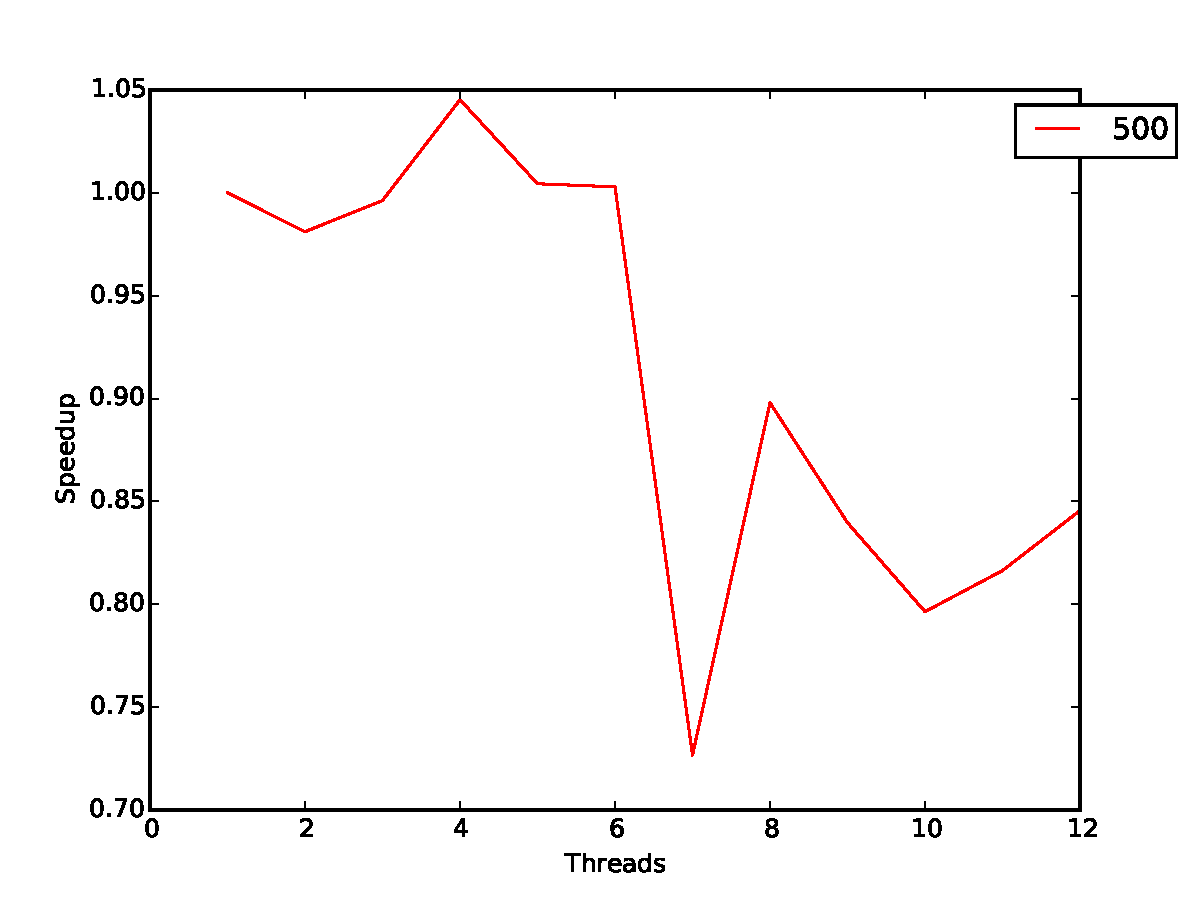
\includegraphics[width=0.5\textwidth]{plots/weak_block-mpi.pdf}
\caption{Weak scaling for block-mpi (baseline of itself).}
\label{weak-block-mpi}
\end{figure}

\subsubsection{Hybrid}

\begin{figure}[ht]
\centering
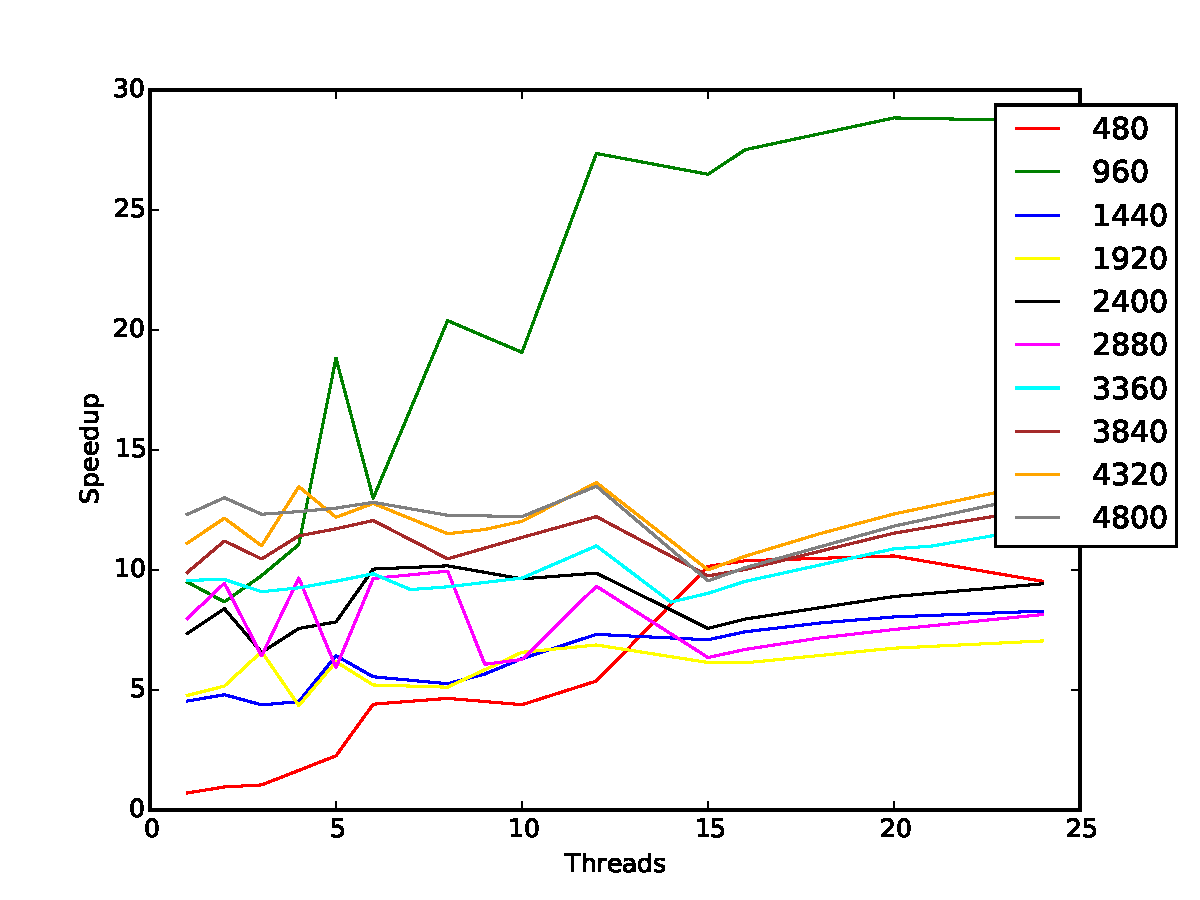
\includegraphics[width=0.5\textwidth]{plots/strong_block-hybrid_baseline-rs-omp--1.pdf}
\caption{Strong scaling for block-hybrid with a baseline of rs-omp}
\label{strong-block-hybrid}
\end{figure}

\begin{figure}[ht]
\centering
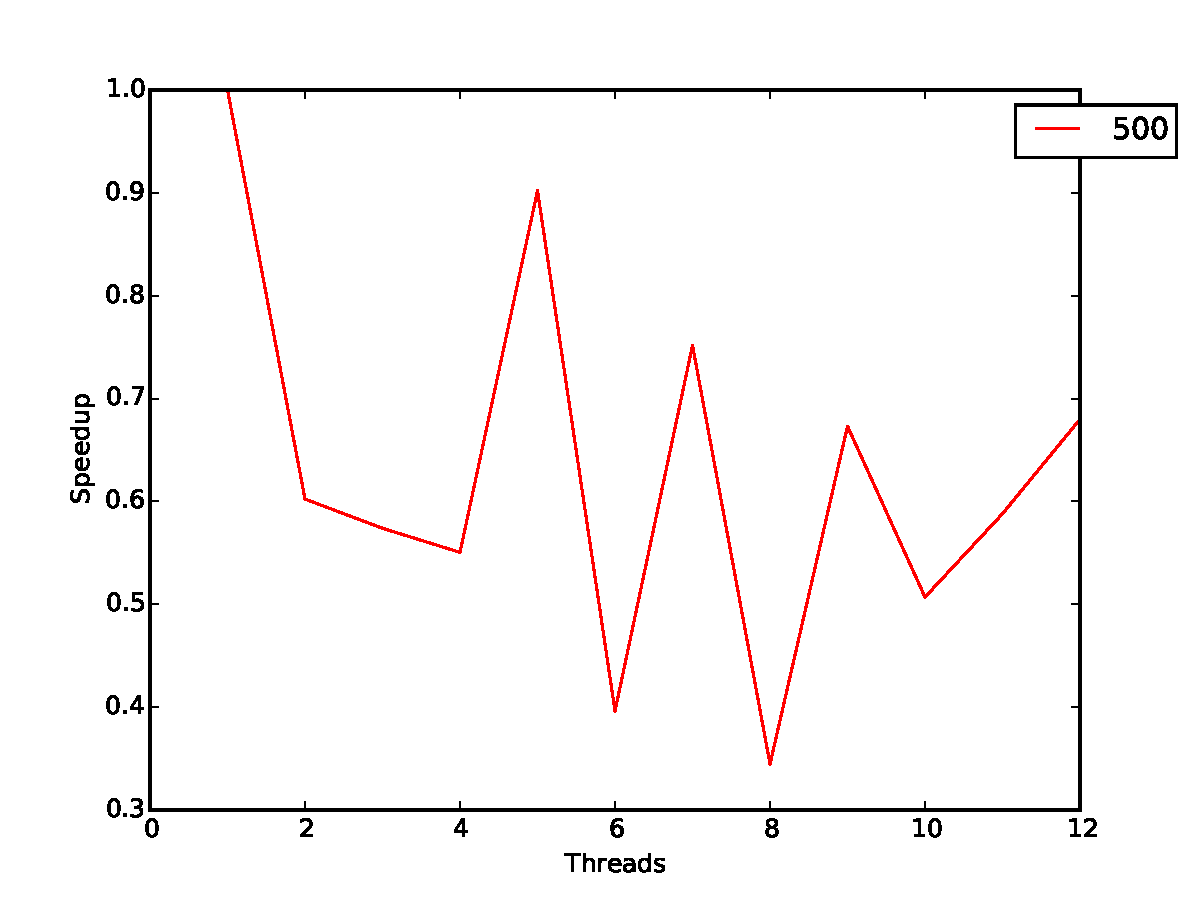
\includegraphics[width=0.5\textwidth]{plots/weak_block-hybrid.pdf}
\caption{Weak scaling for block-hybrid (baseline of itself).}
\label{weak-block-hybrid}
\end{figure}

\subsection{FW}

\subsubsection{MPI}

\begin{figure}[ht]
\centering
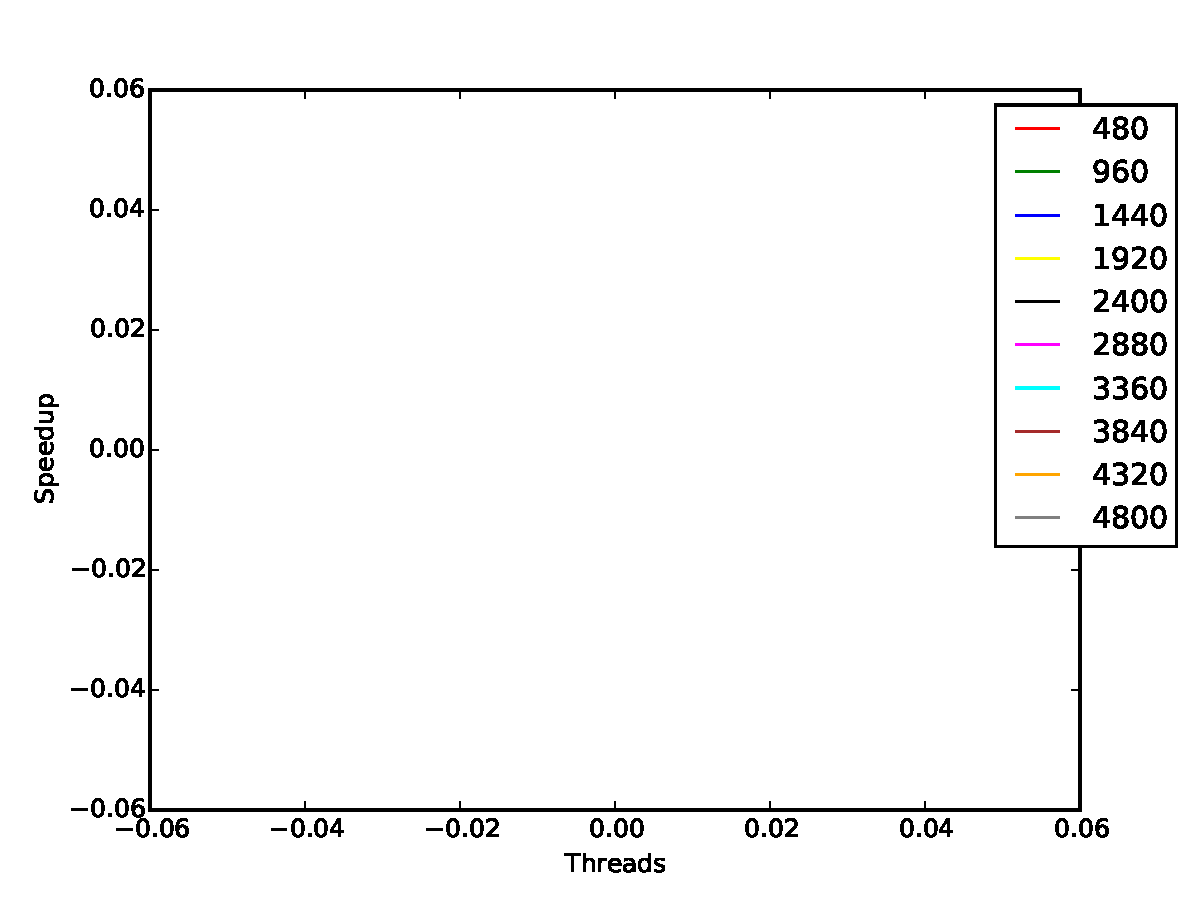
\includegraphics[width=0.5\textwidth]{plots/strong_fw-mpi_baseline-fw-omp--1.pdf}
\caption{Strong scaling for fw-mpi with a baseline of fw-omp}
\label{strong-fw-mpi}
\end{figure}

\subsubsection{Hybrid}

\begin{figure}[ht]
\centering
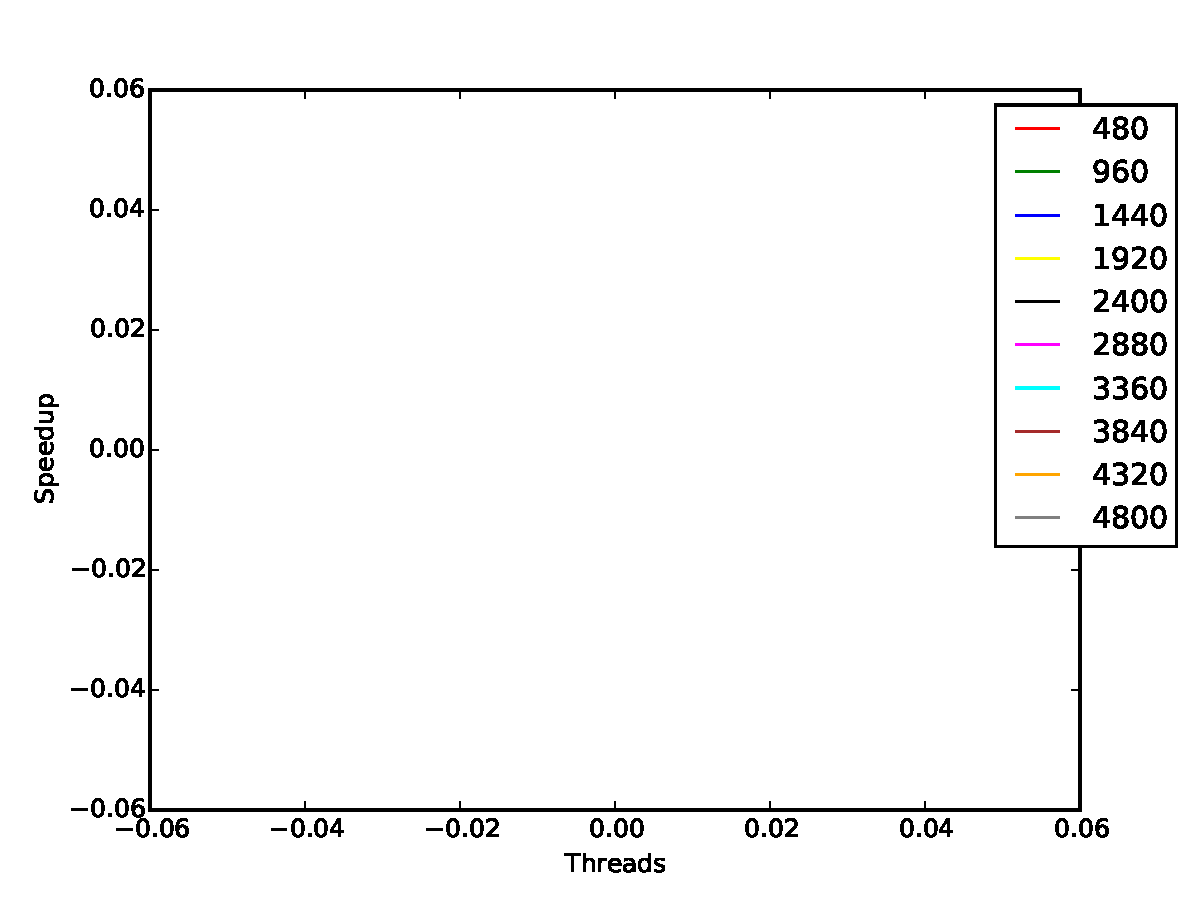
\includegraphics[width=0.5\textwidth]{plots/strong_fw-hybrid_baseline-fw-omp--1.pdf}
\caption{Strong scaling for fw-hybrid with a baseline of fw-omp}
\label{strong-fw-mpi}
\end{figure}

\section{Conclusion}\label{sec:conclusion}


% \section{Tuning}\label{sec:tuning}
We haven't yet spent much time tuning the code serially. The main thing we did
to improve the serial code was to align memory used in \texttt{lnew} and
\texttt{l} along 64-byte boundaries. This allows us to use \texttt{\#pragma
vector aligned} so code is vectorized using aligned instructions instead of
unaligned instructions which are less efficient.

{
\scriptsize
\begin{verbatim}
LOOP BEGIN at path.c(81,5) inlined into path.c(234,5)
   remark #15389: vectorization support: reference l has unaligned access   [ path.c(83,13) ]
   remark #15389: vectorization support: reference l has unaligned access   [ path.c(83,13) ]
   remark #15381: vectorization support: unaligned access used inside loop body
   remark #15300: LOOP WAS VECTORIZED
   remark #15442: entire loop may be executed in remainder
   remark #15450: unmasked unaligned unit stride loads: 1
   remark #15451: unmasked unaligned unit stride stores: 1
   remark #15475: --- begin vector loop cost summary ---
   remark #15476: scalar loop cost: 14
   remark #15477: vector loop cost: 1.750
   remark #15478: estimated potential speedup: 6.140
   remark #15479: lightweight vector operations: 10
   remark #15488: --- end vector loop cost summary ---
LOOP END
\end{verbatim}
}

% \section{MPI}\label{sec:mpi}
\subsection{Implementation}
Implementing this algorithm in MPI requires decomposing the problem into sub
parts, similar to the idea of domain decomposition from the last project. We
drew inspiration from previous work with distance-vector routing using
Bellman$-$Ford in determining shortest distances between routers. In that
algorithm, each router sends its distances to all other routers (each time
there is a change) to its neighbors which then use that information to update
their own distances. This continues until no routers have changed distances.

In our case we do not necessarily have a single thread per node, as there maybe
not be enough available hardware threads. Instead each ''router'' is an MPI
rank and is responsible for a set of nodes rather than a single node. Each MPI
rank calculates the minimum distance to each of its nodes from all other nodes
going through some node between 1 and $N$. Each rank also determines if any
distances have changed. All MPI ranks then synchronize, to gather distances
from one another and determine if any distances have changed (if none stop then
we are done and the ''master'' rank (rank 0) outputs checksum and timing
information). To determine if any distances have changed we use
\texttt{mpi\_allreduce} on each rank's done variable. To synchronize distances
across all ranks we use \texttt{mpi\_allgather} which sends each rank's
distances to all other ranks and collects them from every rank, including
itself, into a single buffer. Our implementation is in \texttt{path-mpi.c}.

\subsection{Performance}
\begin{figure}[h]
  \centering
  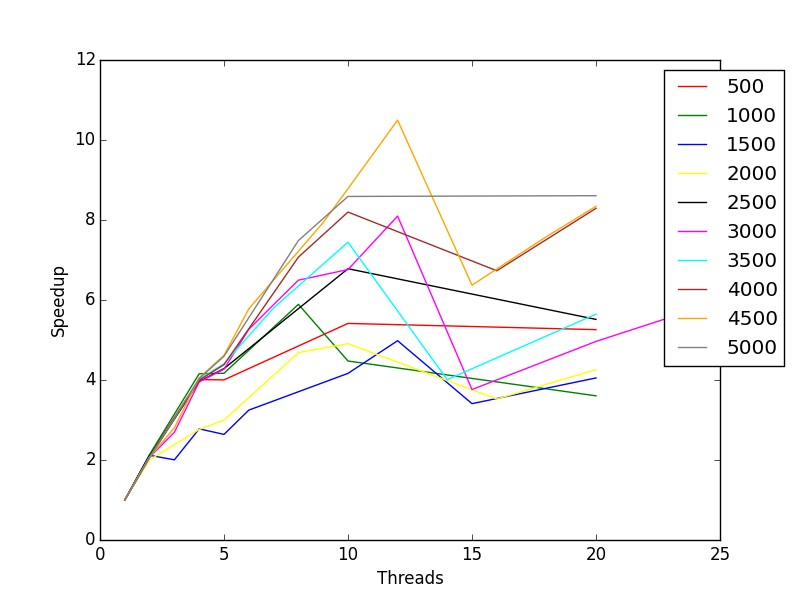
\includegraphics[width=0.68\textwidth] {plots/1}
  \caption{%
    Strong scaling speedup of our MPI code as number of threads (ranks)
    increase. Baseline for calculating speedup is MPI with 1 rank
  }
  \label{aload0}
\end{figure}

\begin{figure}[h]
  \centering
  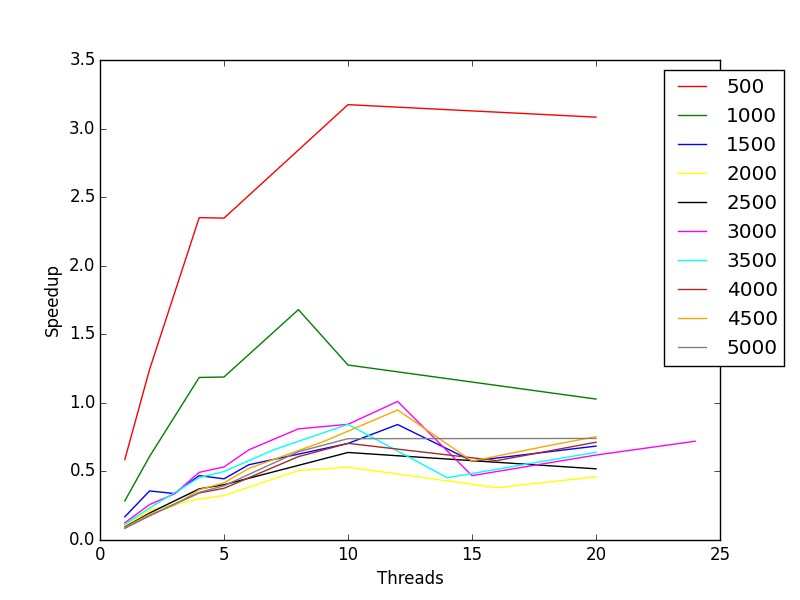
\includegraphics[width=0.68\textwidth] {plots/2}
  \caption{%
    Strong scaling speedup of our MPI code as number of threads (ranks)
    increase. Baseline for calculating speedup is OMP with 24 threads.
  }
  \label{aload1}
\end{figure}

In Figure 1 we show the results of running our MPI code for various problem
sizes and showing how speedup scales as we increase the number of MPI ranks.
Larger problems tend to have greater speedup than smaller ones. This makes
sense as when we increase problem size less time increase spent in
synchronization as compared to actually computation. This means as we increase
the number of ranks we should continue to speedup as synchronization does not
grow as quickly. The drop seen in speedup when we go beyond 12 ranks is due to
now having ranks on 2 chips rather than 1 chip. This increases communication
overhead during synchronization which results in a lower overall speedup
despite having more cores.

We also compared the performance of our MPI code with that of OMP, where omp
was allowed to use all 24 threads (Figure 2) in a strong scaling study. We see
that for the two smallest problem sizes our code outperforms OMP as ranks
increase beyond 1, but for larger problems our MPI code always performs worse.
This is unsurprising as for small problems OMP will have a lot of
synchronization overhead for 24 threads while MPI will do better with a smaller
problem. However, when the problem is larger MPI, which has a larger
synchronization overhead than OMP, MPI performs worse.

% \section{Hybrid (MPI and OMP)}\label{sec:hybrid}
\subsection{Implementation}
MPI and OMP interact seamlessly when put together, making it easy to combine
our MPI implementation and the origin OMP implementation. Given a fixed number
of MPI ranks, $r$, and $p$ available threads then each MPI rank will have
access to $p/r$ threads which can be used in OMP parallel sections of code.
This can mean we do not take full advantage of all threads available to us if
$p$ is not divisible by $r$. We implemented a hybrid version (by combining our
MPI implementation and the OMP parts of the original implementation) in
\texttt{path-mpi-omp.c}

\subsection{Performance}
To study the performance of our hybrid code we did strong scaling studies for a
large range of n and used baselines of our hybride code with 1 MPI rank (Figure
3), our MPI code with 1 MPI rank (Figure 4), and the given OMP code with 24 OMP
threads available (Figure 5).

\begin{figure}[h]
  \centering
  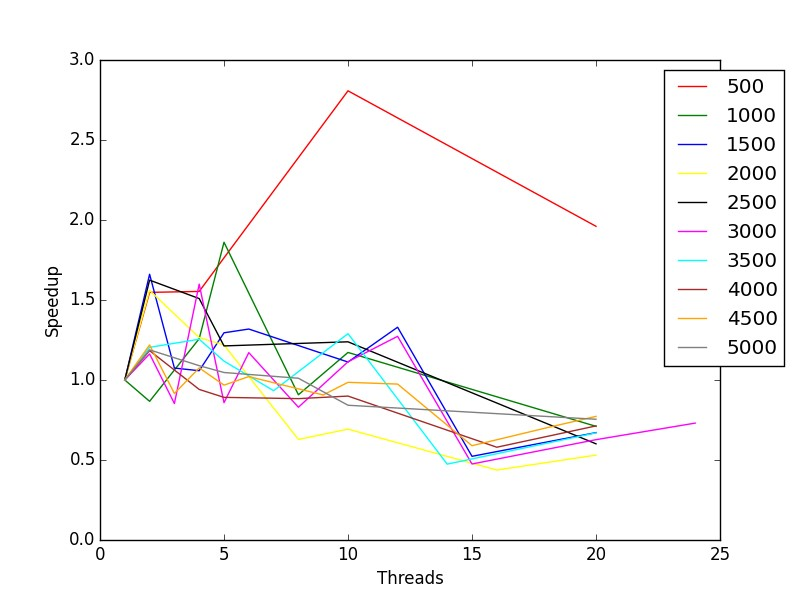
\includegraphics[width=0.63\textwidth] {plots/3}
  \caption{%
    Strong scaling speedup of our Hybrid code as number of MPI ranks increase
    (changing the number of available OMP threads to each rank) increase.
    Baseline for calculating speedup is Hybrid with 1 MPI rank.
  }
  \label{aload0}
\end{figure}
\begin{figure}[h]
  \centering
  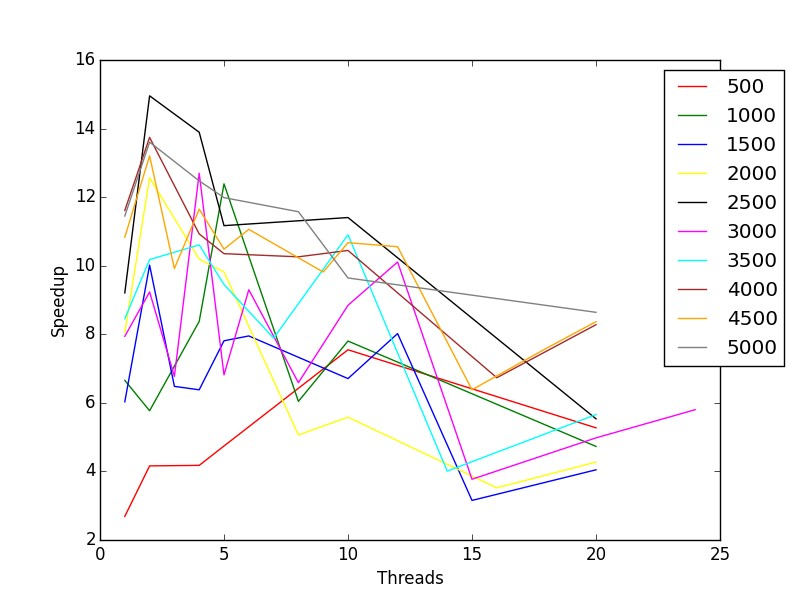
\includegraphics[width=0.63\textwidth] {plots/4}
  \caption{%
    Strong scaling speedup of our Hybrid code as number of MPI ranks increase
    (changing the number of available OMP threads to each rank) increase.
    Baseline for calculating speedup is MPI with 1 MPI rank (thus 1 thread
    total).
  }
  \label{aload1}
\end{figure}

\begin{figure}[h]
  \centering
  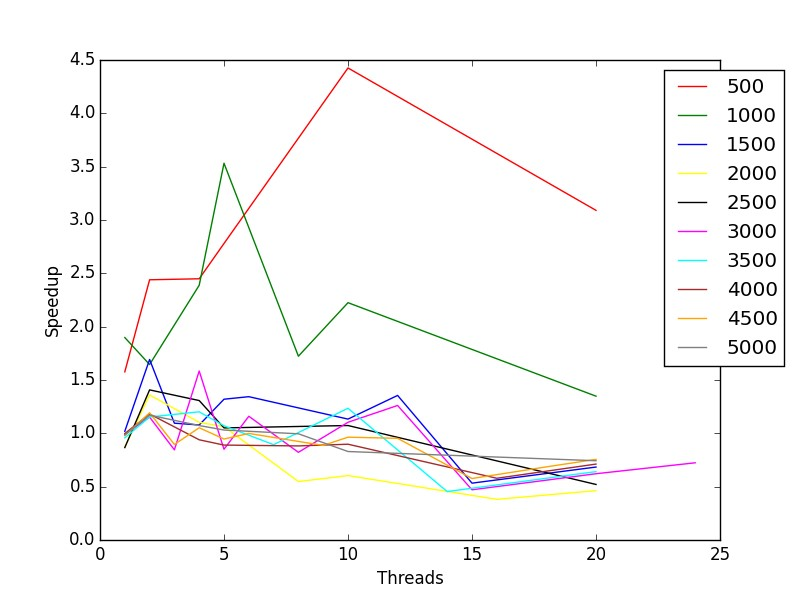
\includegraphics[width=0.65\textwidth]{plots/5}
  \caption{%
    Strong scaling speedup of our Hybrid code as number of MPI ranks increase
    (changing the number of available OMP threads to each rank) increase.
    Baseline for calculating speedup is OMP code with 24 threads.
  }
\end{figure}

In Figure 3 we can see that increasing the number of MPI ranks (which in turn
decreases the number of OMP threads per rank) has mixed speedup for most n.
When the number of MPI ranks is less than 10 we often have speedup larger than
1, but as we go beyond 10 and 12 speedup drops off. This is because of
increased MPI overhead across 2 chips and the hybrid codes inability to take
advantage of all possible threads when there are more than 12 MPI ranks.

In Figure 4 our hybrid code gets large speedup over the (serial) MPI code (1
rank) for all n. This is because mixing MPI and OMP allows the code to take
advantage of more threads than is possible with MPI alone as OMP will take up
remaining threads which aren¡¯t allocated to MPI ranks.

In Figure 5 our hybrid code sometimes manages to get speedup of over 1 as
compared to  the OMP code. This indicates that mixing MPI and OMP can lead to
better thread utilization than using OMP alone.

% \section{Floyd$-$Warshall}\label{sec:fw}
\subsection{Implementation}
The algorithm implemented in the original code runs in $O(\log(N)N^3)$ while
Floyd$-$Warshall runs in $O(N^3)$. This means in theory that Floyd-Warshall
should be significantly faster than the original code. Floyd$-$Warshall is very
similar to the original code, except the loop order is $kij$ (or $kji$), As we
must calculate the shortest distance using all nodes less than or equal to the
current $k$ before calculating for $k+1$. This means the entire set of 3 nested
loops cannot be parallelized. Instead only the inner two can. This decreases
the amount of parallelism and increases the frequency with which data must be
synchronized, while decreasing overall work. We implemented Floyd$-$Warshall (a
rather simple set of changes to the original implementation) in both OMP and
MPI. Our implementations are in \texttt{fw-omp.c} and \texttt{fw-mpi.c}
respectively.

\subsection{Performance}
\begin{figure}[h]
  \centering
  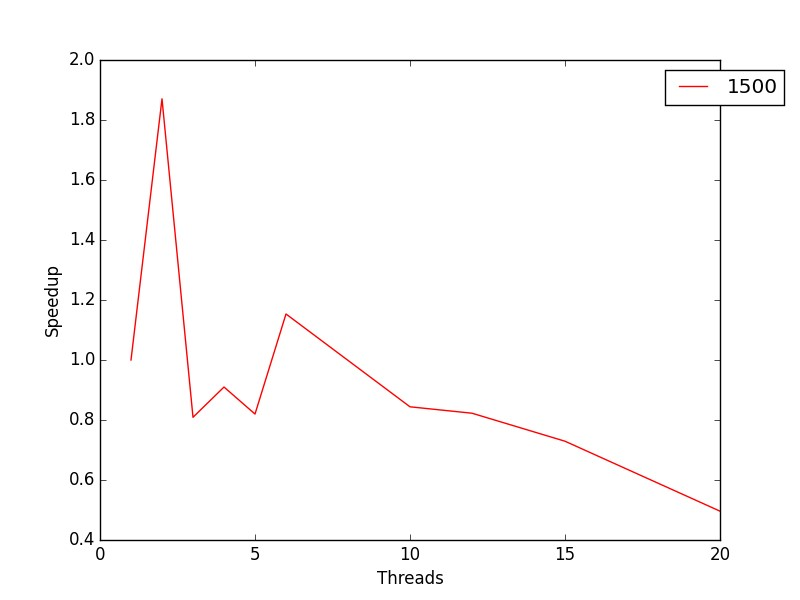
\includegraphics[width=0.68\textwidth] {plots/6}
  \caption{%
    Strong scaling speedup of our Floyd$-$Warshall MPI code as number of MPI
    ranks increases. Baseline for calculating speedup is Floyd-Warshall MPI
    code with 1 rank.
  }
  \label{aload0}
\end{figure}
\begin{figure}[h]
  \centering
  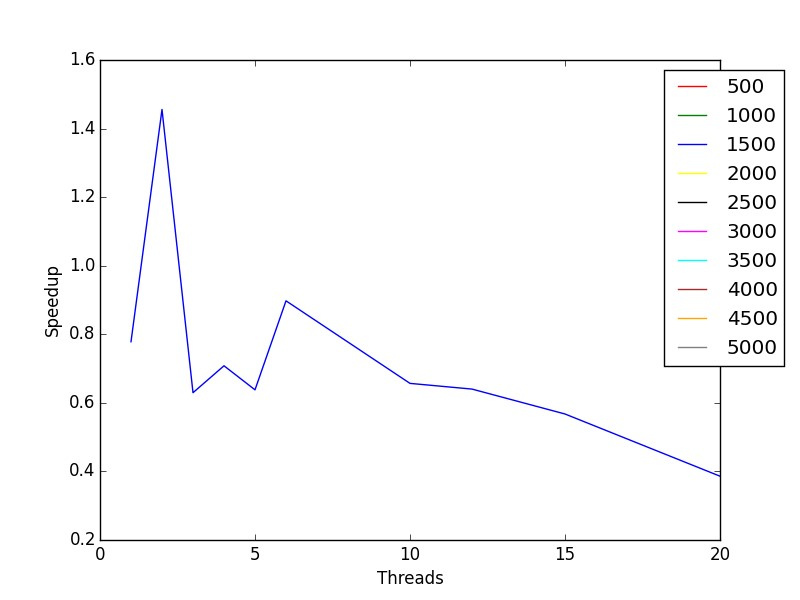
\includegraphics[width=0.68\textwidth] {plots/7}
  \caption{%
    Strong scaling speedup of our Floyd$-$Warshall MPI code as number of MPI
    ranks increases. Baseline for calculating speedup is our original MPI code
    with 1 rank.
  }
  \label{aload1}
\end{figure}

We tested our Floyd$-$Warshall code for a single $n$ (1500), as it does not
scale well. We calculated strong scaling for this $n$ using a baseline of the
Floyd$-$Warshall MPI code with 1 rank (Figure 6) and a baseline of our original
MPI code with 1 rank (Figure 7). In Figure 6, the performance of FW MPI
increases only until 2 and then starts to drop off. This is for two reasons:
the first is the increased overhead once we go beyond 12 ranks (communication
across 2 chips is slower) and the larger reason is that communication is
expensive in Floyd$-$Warshall. Because we have to synchronize $O(N)$ times
rather than $O(\log(N))$ times as we increase the amount of communication that
is done (by increasing number of ranks) we see that our code gets slower as we
add more parallelism.

In Figure 7 we can see that our speedup is even smaller when compared to our
original MPI code, for the exact same reason as before: The extra communication
is a major cost and results in a decline in performance as rank increases.


\end{document}
